% Configuração da fonte Fira Code
%\usepackage{FiraMono}

%\usepackage{caption}

\newcommand{\danger}{\faIcon{exclamation-triangle}}

% Configuração da fonte para a descrição
\newcommand{\descfont}{\fontfamily{cmss}\selectfont}

%\usepackage{listings}

% Configuração da fonte para comandos na shell
\lstset{
    basicstyle=\ttfamily\small, % Escolha a fonte desejada para os comandos
    breaklines=true,
    showstringspaces=false,
    literate=
        *{\#}{{\textcolor{cyan}{\#}}}1
        {\@}{{\textcolor{purple}{@}}}5
        {\{}{{\textcolor{purple}{\{}}}1
        {\}}{{\textcolor{purple}{\}}}}1
    ,
    stringstyle=\color{purple},
    keywordstyle=\color{blue}
}


\chapter{Analysis and Requirement Specification}\label{chap:chap3}

This chapter presents a detailed description of the work developed through the internship.\newline

\begin{tcolorbox}[colback=white!20!white,colframe=red!80!black,rounded corners]
\danger The \textit{entirety of the projects presented} on this chapter can be seen \href{https://github.com/BrunaMacieira/Internship/tree/main}{here}\footnotemark.\danger\newline
\end{tcolorbox}

\footnotetext{The URL for the repository is: https://github.com/BrunaMacieira/Internship/tree/main}

\section{Work Introduction}

Extensive analysis and requirement specification have been conducted to ensure the successful implementation of Dharma Network. The platform's architecture, security measures, scalability and usability have been thoroughly evaluated to meet the needs of users and provide a seamless DeFi experience. \newline

Taking Dharma Network as the basis, it has one major actor: the user. The user can be a developer, a non-developer (such as marketing team, designer, etc) and/or the responsible for the organization.

The user must have a wallet from Pera Wallet, MyAlgo wallet, AlgoSigner, WalletConnect or any other Algorand compatible wallet. Users are identified by their wallet address.\newline

The Product backlog for the user can be set as following \cite{dharma}:

\begin{itemize}
	\item as a User, I want to connect a wallet
	\item as a User, I want to update my profile so I can update my personal information, such as email, phone, username or profession
	\item as a User, I want to create an organization
	\item as a User, I want to join an organization
	\item as a User, I want to invite someone to join an organization
    \item as a User, I want to fund organizations with funding rounds in Algo or Dharm
    \item as a User, I want to manage multiple organizations simultaneously
    \item as a User, I want to create and join multiple projects inside each organization
    \item as a User, I want to track automated activity on multiple projects for developers
    \item as a User, I want to add manual tracking of activity for non-developers
    \item as a User, I want to get statistics and information of multiple projects inside the organization
    \item as a User, I want to give and receive feedback on a project
    \item as a User, I want to vote on the weight each activity type has in work units
    \item as a User, I want to get rewarded by mining Dharm based on the work I've done
	\item as a User, I want to get additional mining by holding Dharm during a funding round
    \item as a User, I want to inspect blocks and the rewards distribution
	
\end{itemize}

In this initial phase, the process of learning was mandatory, since there was no previous contact with functional programming or blockchain. \newline

\section{Études for Elixir}

The very first skill required was to learn Elixir. As previously mentioned, Elixir is a colossal part of Dharma Network, so it made sense to start from here.

Yarilabs has experience teaching this functional programming language, since they host summer internships nearly every year, so they had the material set: the \textit{Études for Elixir}.

The \emph{Études for Elixir} (Eisenberg, 2014) consists of a compilation of exercises, slowly increasing the level of difficulty. 

The exercises are not usually extensive and each one belongs to a chapter related to an Elixir concept. During the completion of the tasks, the student is advised to read support material, specifically \emph{Introducing Elixir} \cite{elixir}.\newline

As an extension of the content seen on section \ref{elixir}, for the development of the \textit{Études for Elixir}, Elixir needs to be installed, depending on the operative system in question. Then, a project can be created: \newline

{
\newcommand{\shellcmd}[1]{\\\indent\indent\texttt{\footnotesize\# #1}\\}
  \shellcmd{mix new demo --module Demo}
}

This command uses \textit{Mix build tool}, which comes bundled with the language. Mix simplifies project creation and management by providing a set of predefined tasks and conventions. It generates a new Elixir project structure, including directories for source code, tests and dependencies (see section \ref{elixir}). \newline

The \textit{Études} are divided into 13 chapters, specifically:

\begin{enumerate}

    \item first Elixir code, with errors
    \item functions and modules
    \item tuples and records
    \item logic and recursion
    \item strings
    \item lists
    \item hashes
    \item higher order functions and list comprehensions
    \item processes
    \item errors
    \item storing structured data
    \item OTP
    \item macros
    
\end{enumerate}

Luckily, while learning and developing these, snippets of code were debated with a teammate, João Martins, a Frontend developer for Dharma Network, whom had the courage to learn Elixir and gain more skills. Thanks to him, more algorithm alternatives were provided during this process.

\subsection{Development of Études for Elixir}

The exercises of \textit{Études for Elixir} can be found on O'Reilly's \href{https://github.com/oreillymedia/etudes-for-elixir/tree/master}{\textbf{GitHub page}}\footnote{Études for Elixir can be found on: https://github.com/oreillymedia/etudes-for-elixir/tree/master}.\newline


By immersing themselves in these practices, developers acquire a deeper understanding of Elixir's syntax, features, and idioms, enabling them to write more robust and maintainable code. They also gain insights into code organization, module design, and the functional programming paradigm, which can enhance their overall programming skills. Additionally, developers can learn valuable techniques for debugging, testing, and optimizing Elixir applications, improving their ability to deliver high-quality software solutions. 

\section{Fake Twitter with Phoenix Framework}

After learning the basics of Elixir, the next step is to move onto Phoenix, the framework that incorporates Elixir.

Working with Phoenix is an adventure, because a developer doesn't feel fatigued for always working with the same language; that's because it doesn't happen.

Phoenix passes the experience of working as a full-stack developer without the need of being one.

As for the first dive into the Phoenix world, it consisted of the mimic of a worldwide known application: Twitter.

Twitter's basic characteristics are: posting, liking, reposting, deleting and updating a tweet, all in real time. Of course that an account needs to be created and the user can update their profile, but the main principle to be taken from this project was the connection between the pages.

The creation of a project using Phoenix is extremely simple: \newline

{
\newcommand{\shellcmd}[1]{\\\indent\indent\texttt{\footnotesize\# #1}\\}
    \shellcmd{mix archive.install hex phx\_new}
    \shellcmd{mix phx.new fake\_twitter}
}

This will create a project named \texttt{fake\_twitter}. \newline

When a project is created and it's connected to a port (default port is 4000), Phoenix's front page will be displayed, as seen on figure \ref{fig:phoenix}:

\begin{figure}[htbp]
	\centering
	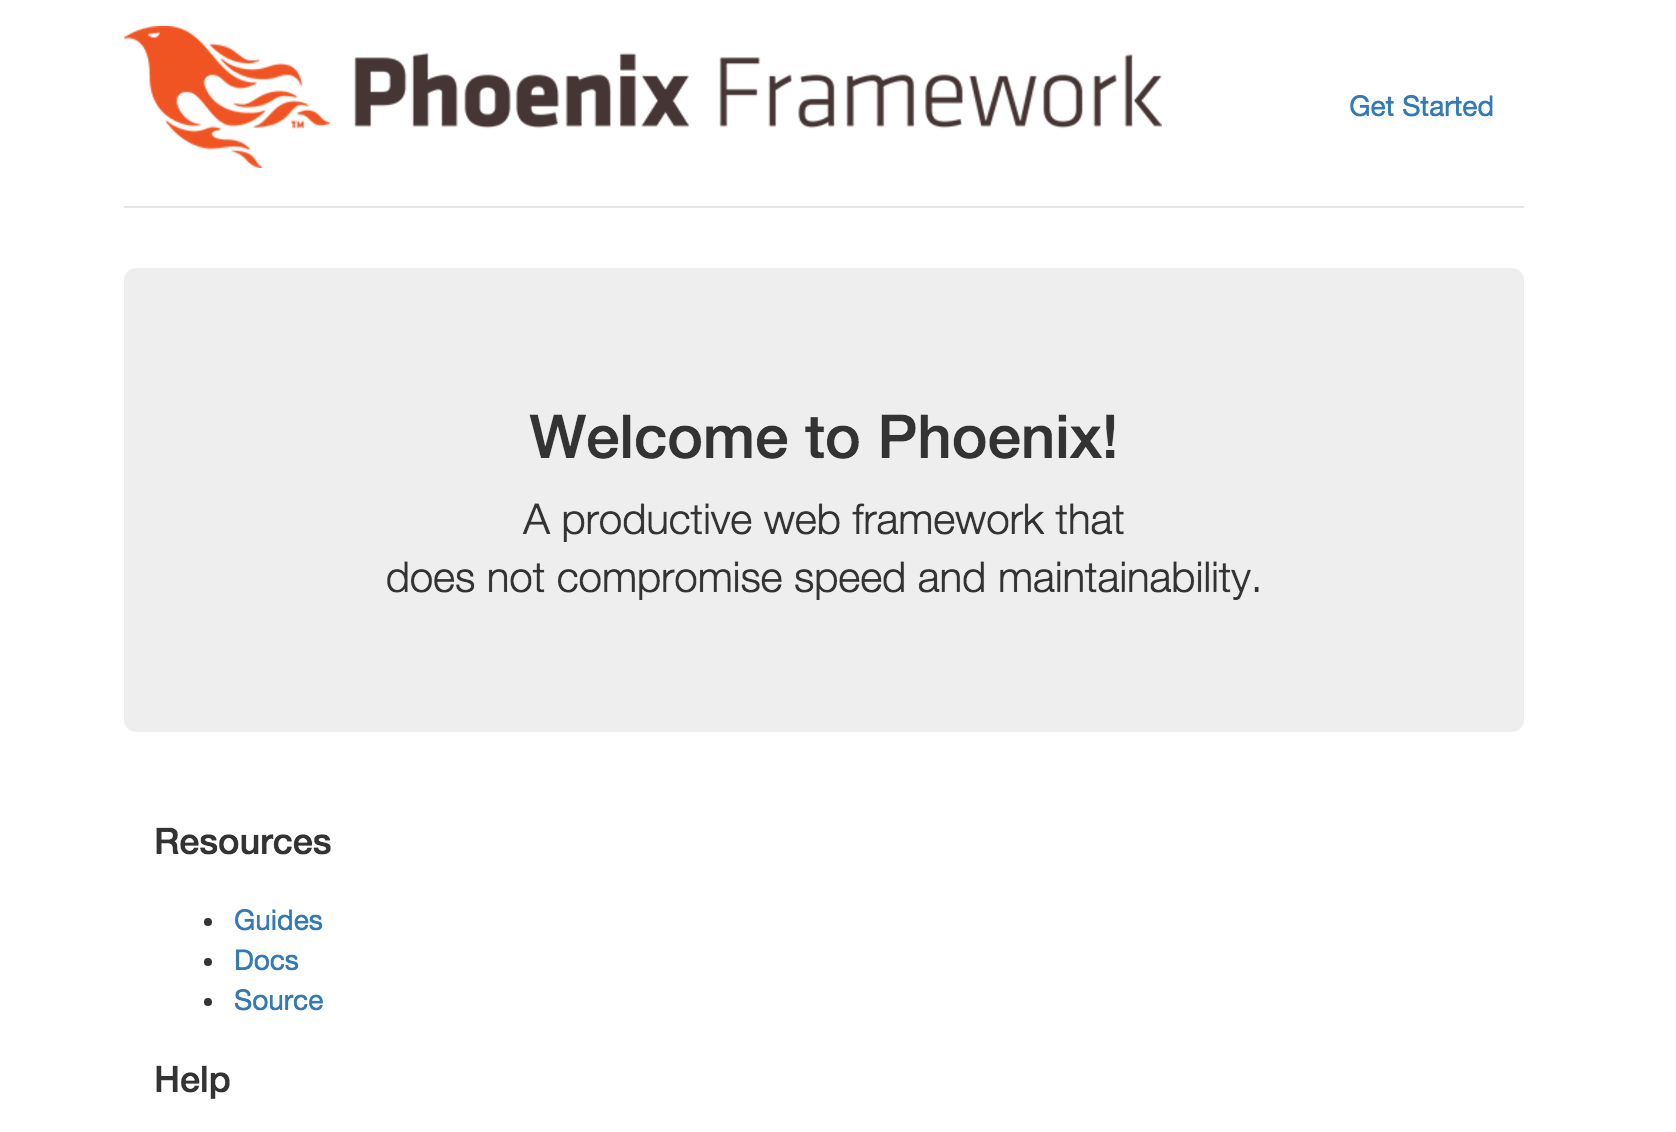
\includegraphics[width=1\linewidth]{figures/phoenix_welcome_page.png}  % largura percentual
	\caption{Phoenix Front Page}
	\label{fig:phoenix}
\end{figure}

Looking at the body of the project, it has built-in generated folders and scripts:

\begin{itemize}
    \item a folder named "assets"
    \item a folder named "config"
    \item a folder named "lib"
    \item a folder named "priv"
    \item a folder named "test"
    \item dependancy files, such as "mix.exs", "mix.lock"
    \item README.md and .gitignore files
\end{itemize}

\begin{figure}[htbp]
	\centering
	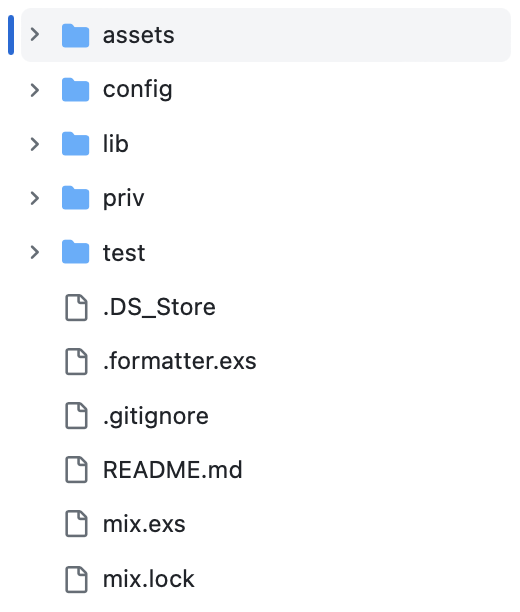
\includegraphics[scale=0.5]{figures/phx-folders.png}  % largura percentual
	\caption{Phoenix Generated Files}
	\label{fig:phx}
\end{figure}

"Assets" folder contains the information responsible for the style of the application, like CSS and JavaScript files.

"Config" folder guards the necessary paths to connect the application, as well as signing salt and other cryptography information.

"Priv" folder contains the seeds file, migrations and static characteristics, like images.

"Test" folder, as the name says, stores automatic and manual tests than run in order to guarantee the safety and maintainability of the application.

"Lib" folder is probably the most important one of them all, since it stores two folders: \texttt{fake\_twitter} and \texttt{fake\_twitter\_web}. Each one of these folders has an \texttt{.ex} file related to it, which is the entrypoint for defining the application, such as web controllers, views, channels and everything that's necessary.

\begin{figure}[htbp]
	\centering
	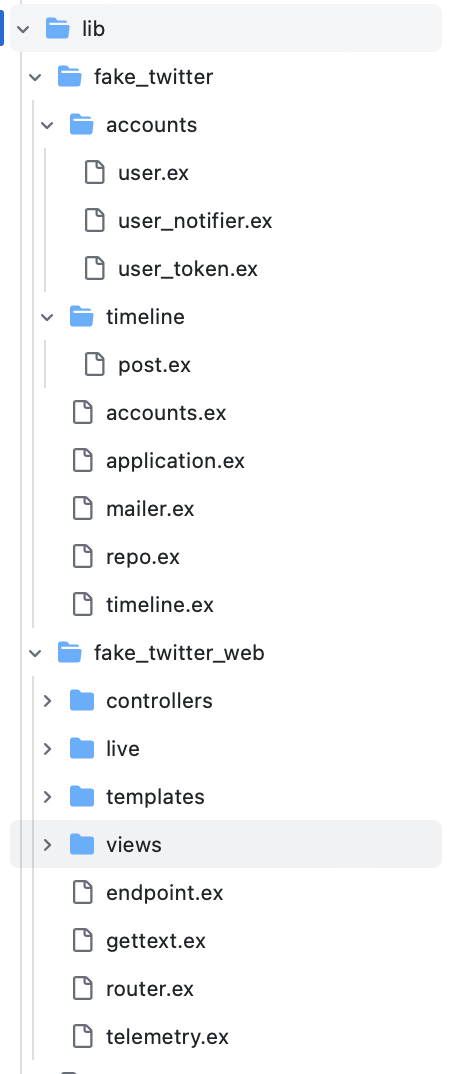
\includegraphics[scale=0.5]{figures/lib.png}  % largura percentual
	\caption{Lib folder}
	\label{fig:phx}
\end{figure}

As it's clear to say, code organization plays a big role in Phoenix, since its folder structure is well divided and pristine. 

The directory \texttt{fake\_twitter} holds the core logic of the application. It includes modules responsible for business logic, data manipulation and domain-specific functionality. The project-specific code resides within this directory, and developers can organize it into subdirectories based on their application's structure.


However, inside \texttt{fake\_twitter\_web} directory, it focuses on the web-specific aspects of the Phoenix application. It contains:

\begin{itemize}
    \item \textit{Controllers}: This directory contains the controllers responsible for handling incoming requests, processing data and generating responses. Controllers are modules that define actions corresponding to different routes, implementing the application's business logic.
    \item \textit{Views}: The \texttt{views} directory holds the modules responsible for rendering templates and generating responses. Views provide a separation of concerns by handling the presentation layer, allowing developers to focus on generating the appropriate response format (e.g., HTML, JSON).
    \item \textit{Templates}: This directory stores the \textit{EEx} templates used by the views. \textit{EEx} is Phoenix's embedded Elixir templating engine, enabling dynamic content generation within HTML, XML or other response formats.
    \item \textit{Static Assets}: The \texttt{static} directory contains static assets such as JavaScript, CSS, images and other files used by the client-side of the application.
    \item \textit{router.ex}: The \texttt{router.ex} file defines the routing configuration for the application. It maps incoming HTTP requests to the appropriate controller actions using a declarative DSL (Domain-Specific Language) provided by Phoenix.
    \item Other files and folders necessary for the correct architecture of the application, such as helpers, error handlers and more.
\end{itemize}

Of course, the user can choose whether they want to add or delete some files/folders. For instance, Phoenix's default database is the relational database PostgreSQL. The user, however, can choose not to create a database or to use another one. But, for its practicality, the default database was used during this project.\newline

The project's features are shown in the figures:

\begin{figure}[htbp]
	\centering
	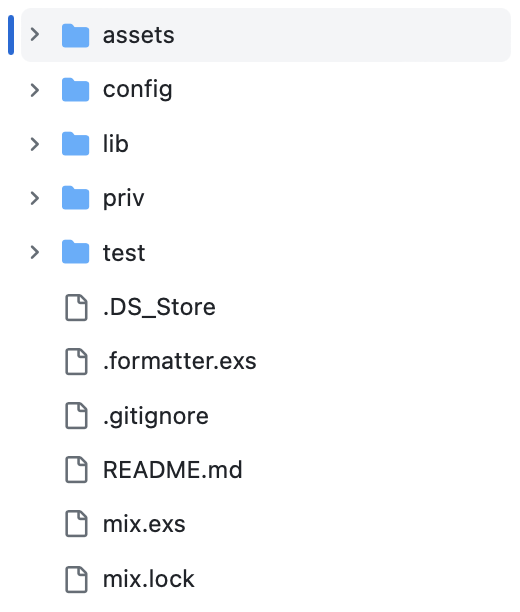
\includegraphics[scale=0.5]{figures/phx-folders.png}  % largura percentual
	\caption{Phoenix Generated Files}
	\label{fig:phx}
\end{figure}



\begin{figure}[htbp]
	\centering
	
	\begin{minipage}[b]{0.45\textwidth}
		\centering
		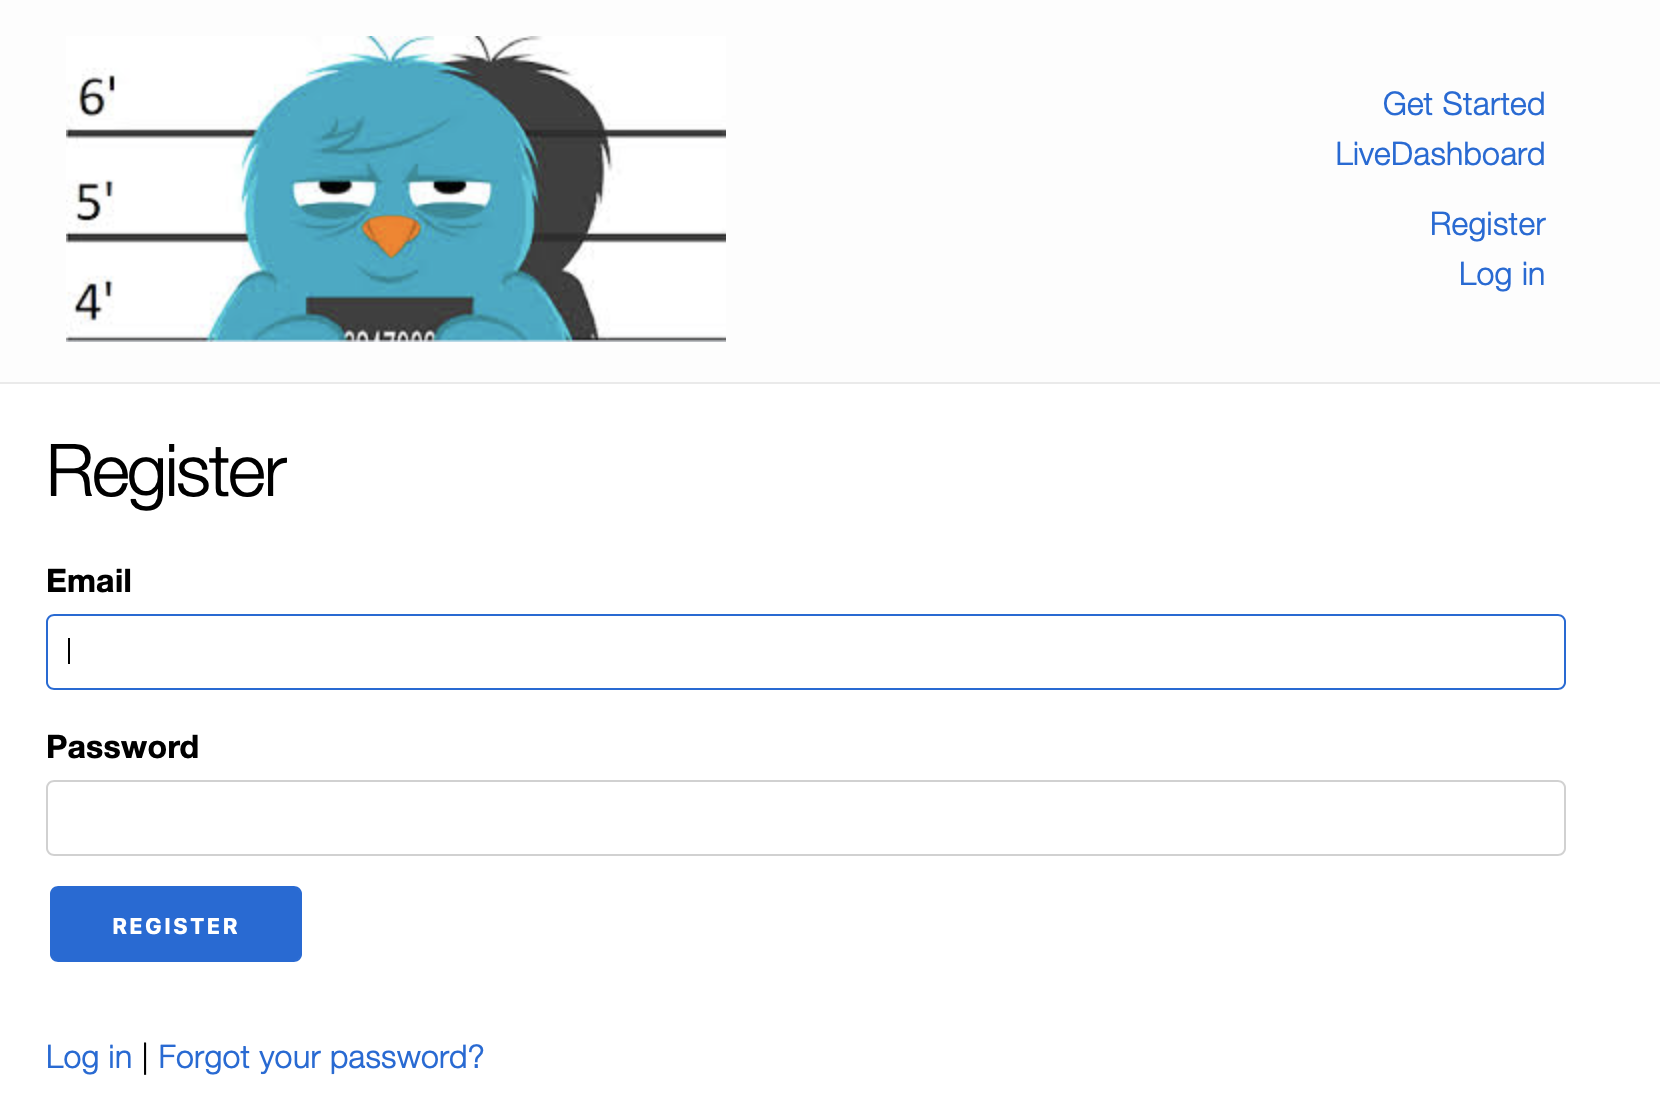
\includegraphics[width=\linewidth]{figures/FT_register.png}
		\caption{Register User}
		\label{fig:register}
	\end{minipage}
	\hfill
	\begin{minipage}[b]{0.45\textwidth}
		\centering
		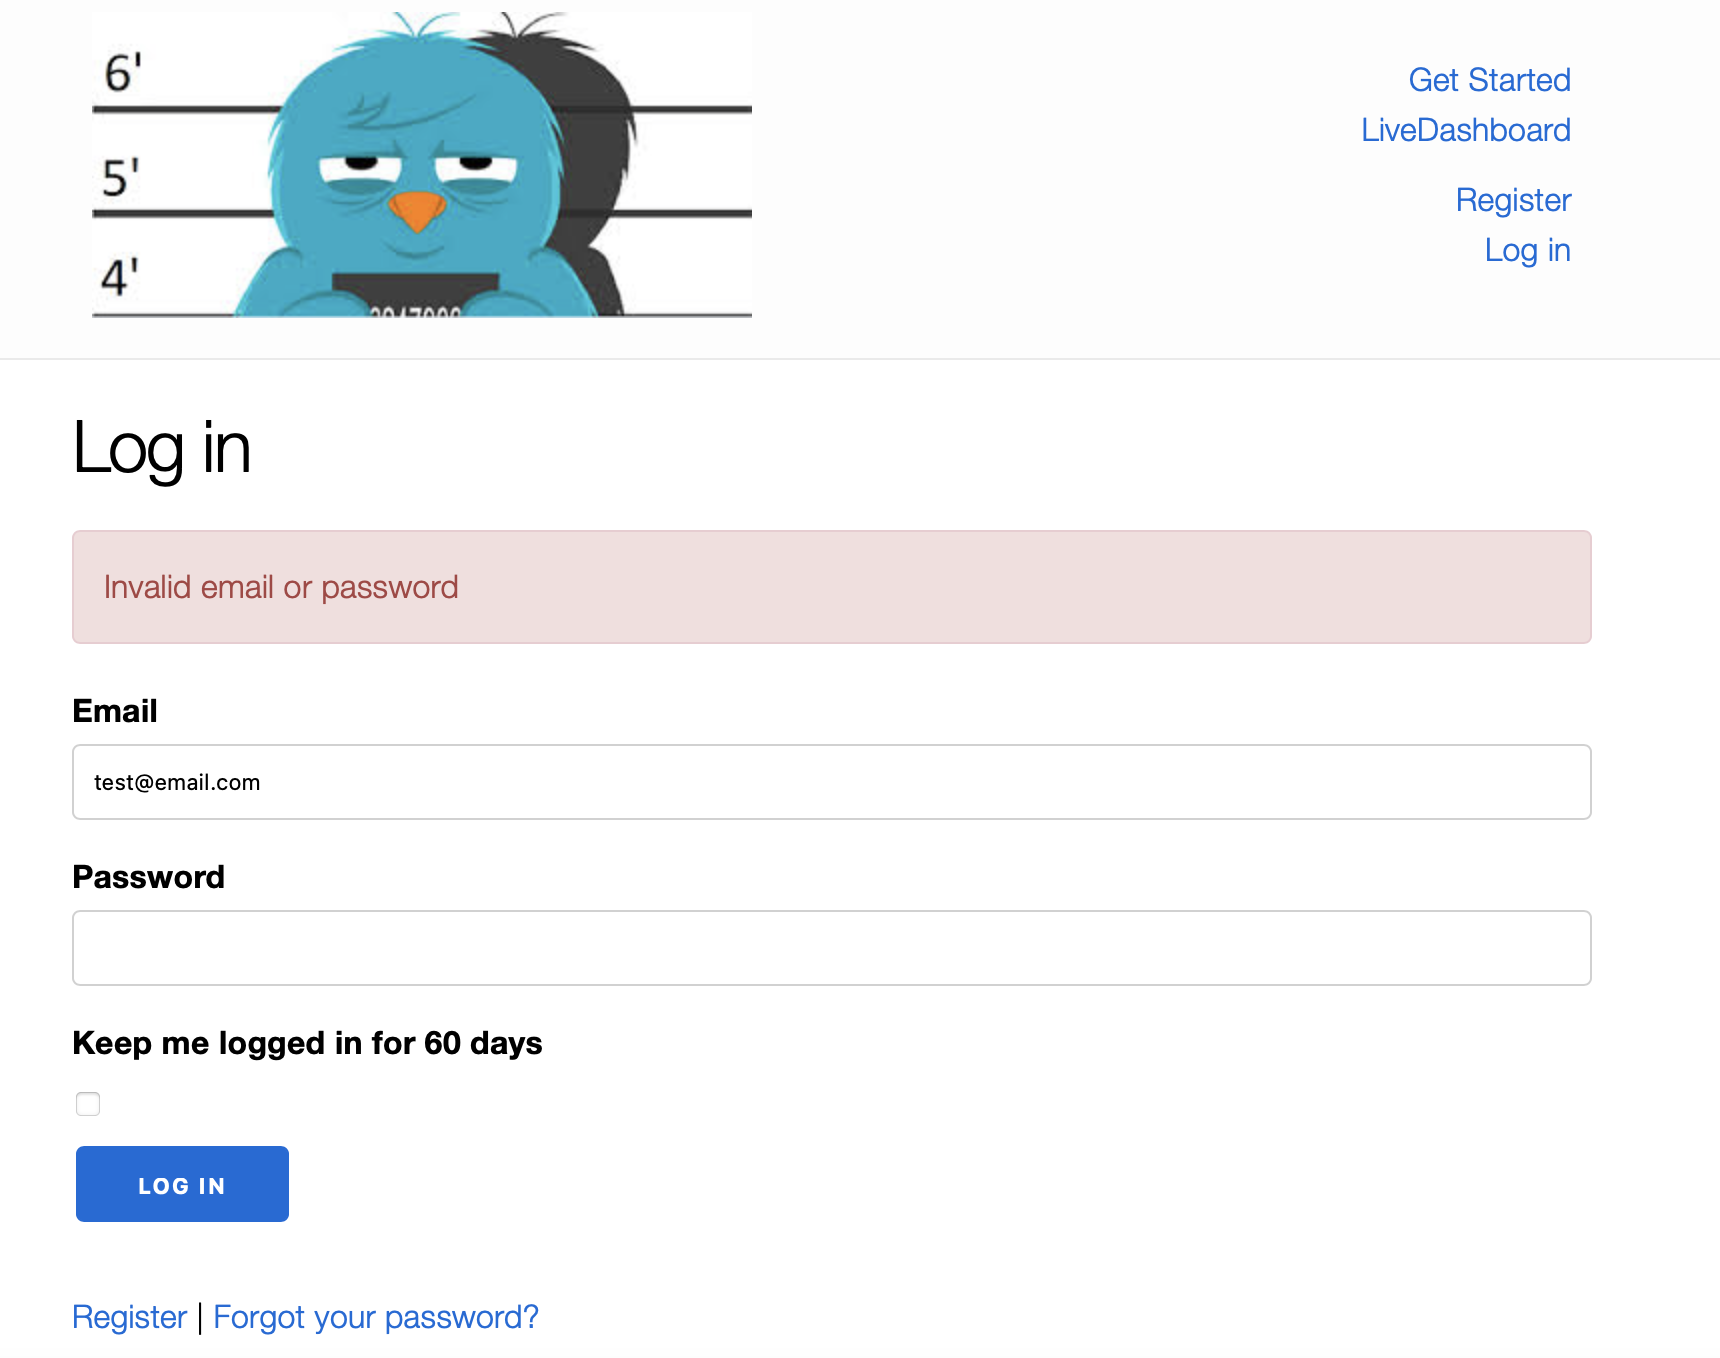
\includegraphics[width=\linewidth]{figures/inv_email.png}
		\caption{Invalid Email}
		\label{fig:inv}
	\end{minipage}

\end{figure}

\begin{figure}[htbp]
	\centering
	
	\begin{minipage}[b]{0.45\textwidth}
		\centering
		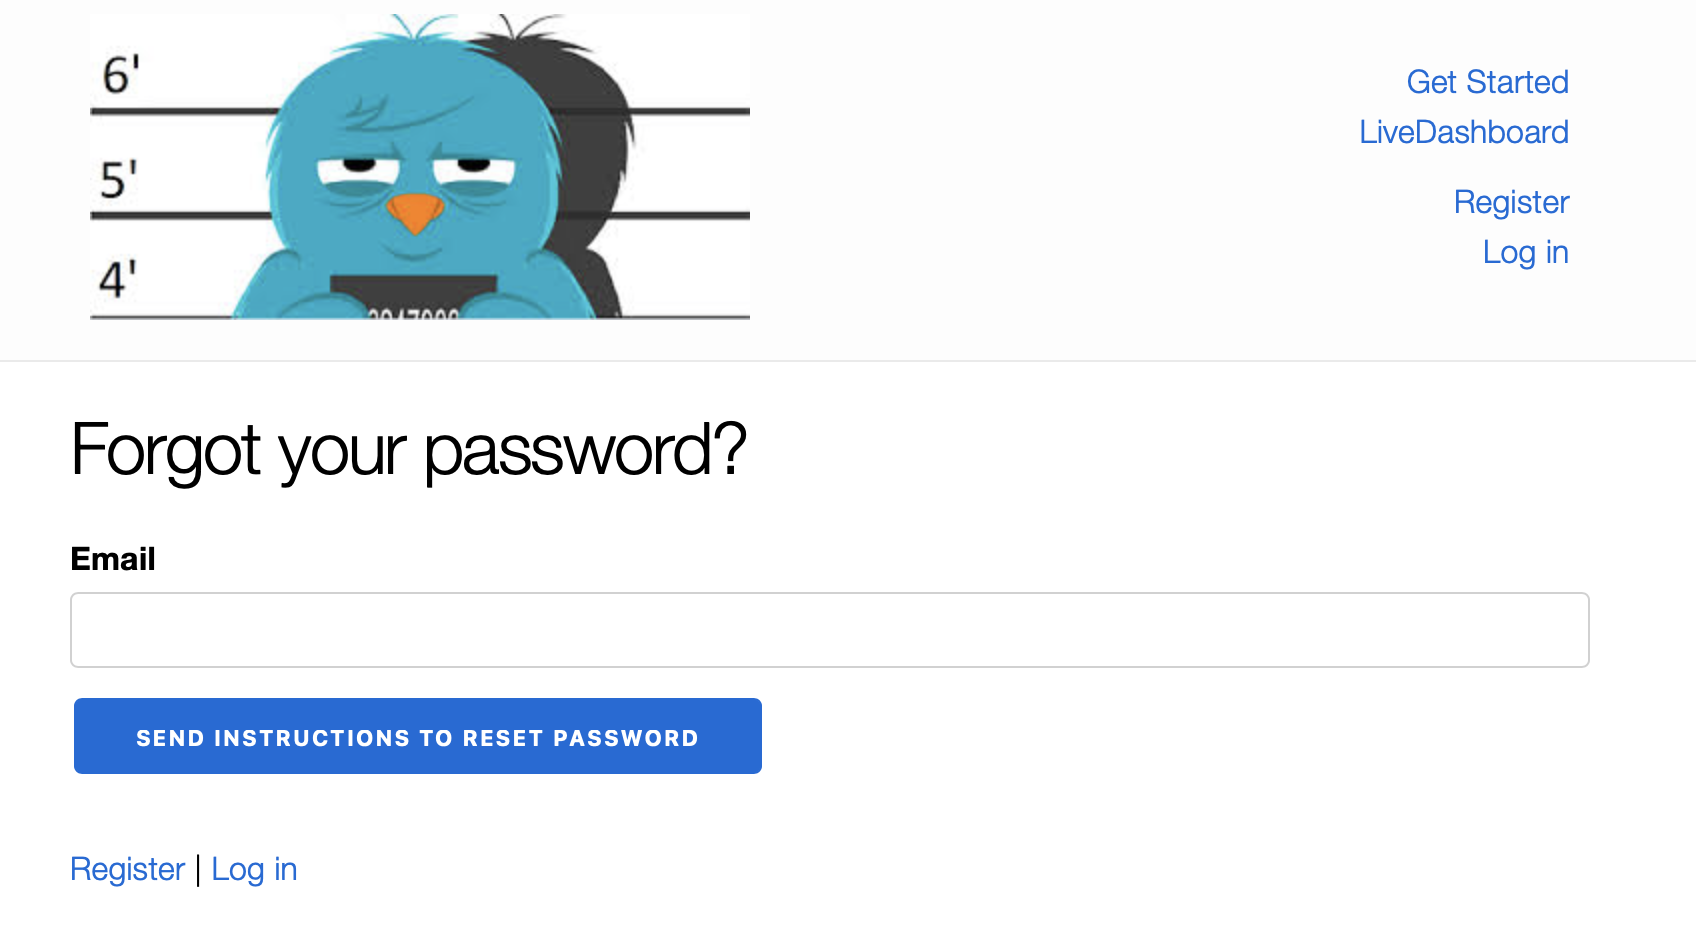
\includegraphics[width=\linewidth]{figures/FT_forgot_pw.png}
		\caption{Forgot Password}
		\label{fig:pw}
	\end{minipage}
	\hfill
	\begin{minipage}[b]{0.45\textwidth}
		\centering
		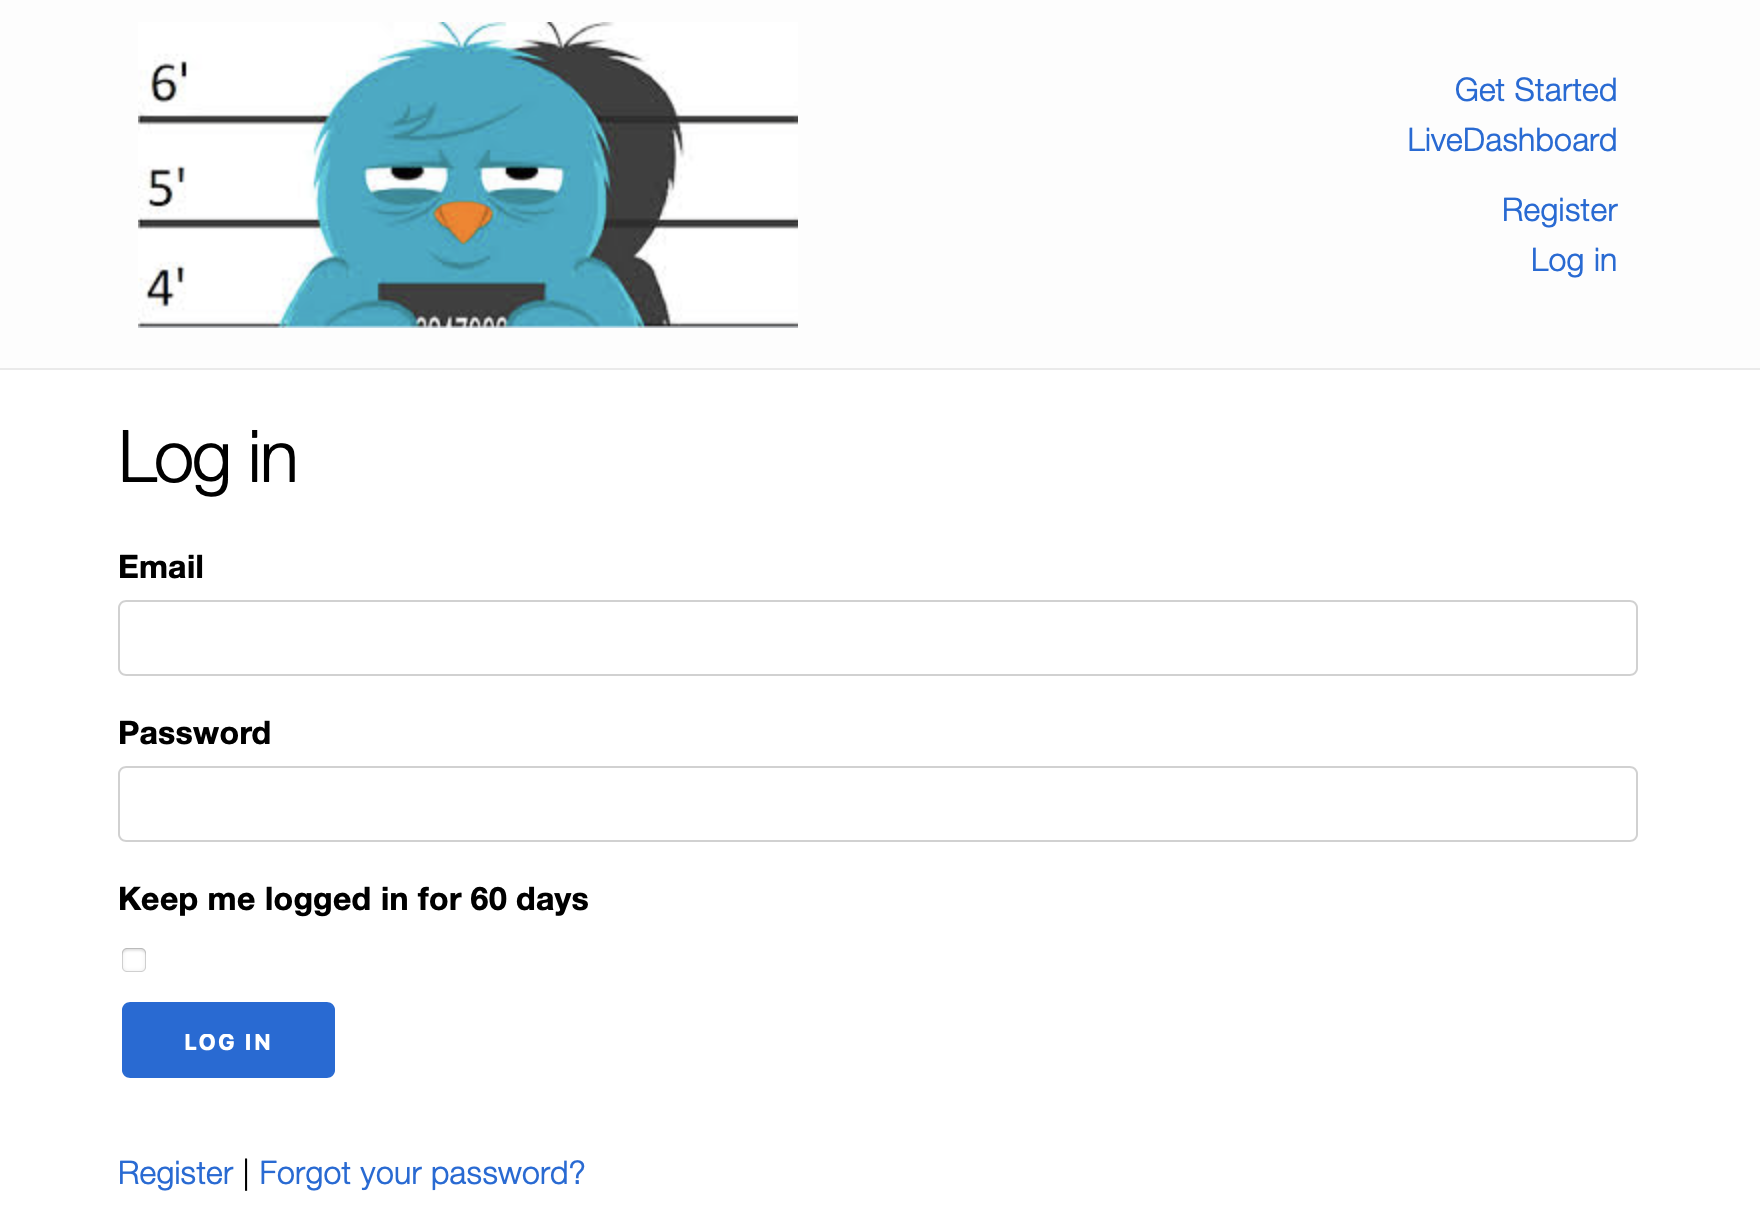
\includegraphics[width=\linewidth]{figures/FT_login.png}
		\caption{Login}
		\label{fig:login}
	\end{minipage}

\end{figure}

\begin{figure}[htbp]
	\centering
	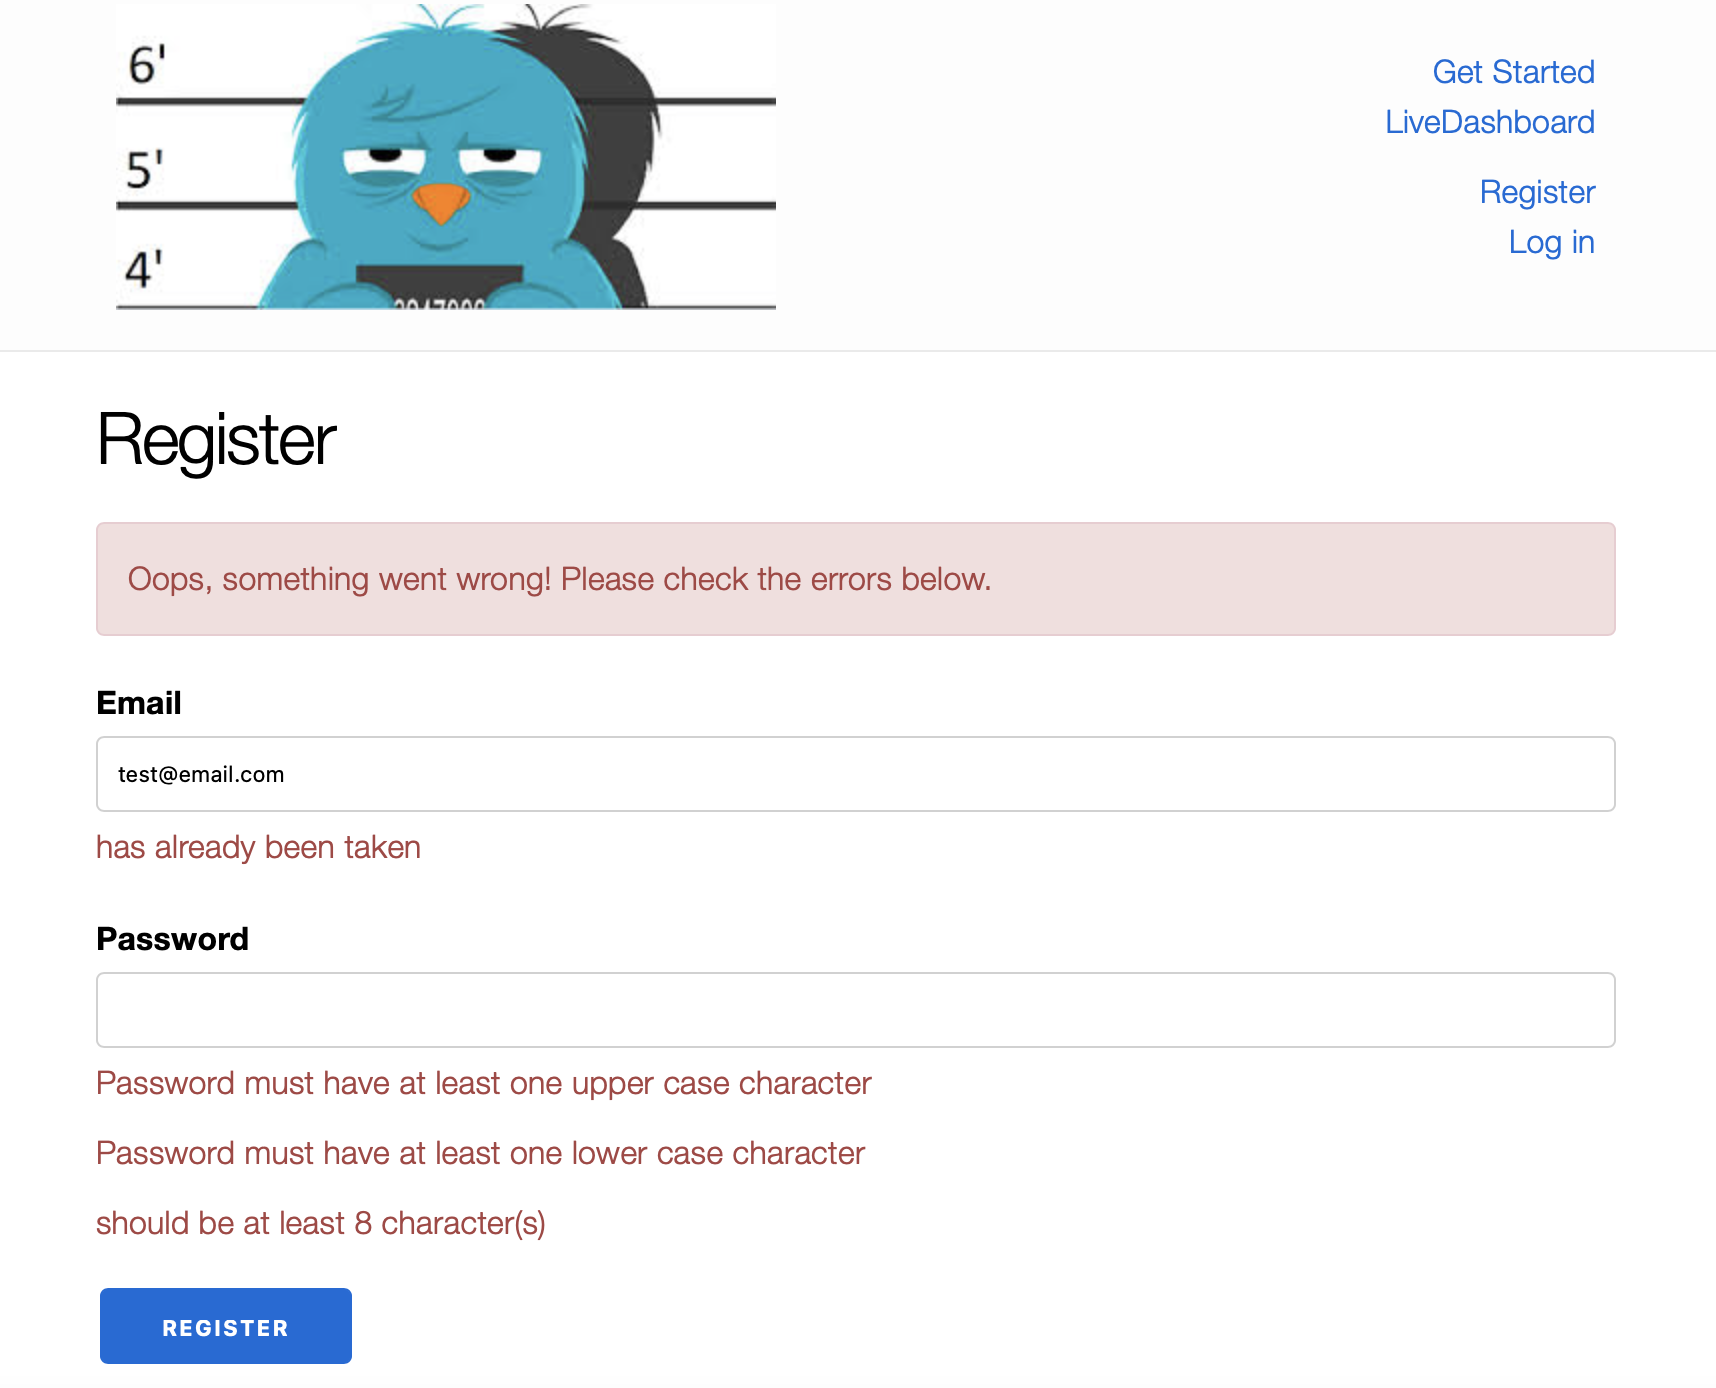
\includegraphics[scale=0.25]{figures/sec.png}  % largura percentual
	\caption{Security features when creating an account}
	\label{fig:sec}
\end{figure}


\begin{figure}[htbp]
	\centering
	
	\begin{minipage}[b]{0.45\textwidth}
		\centering
		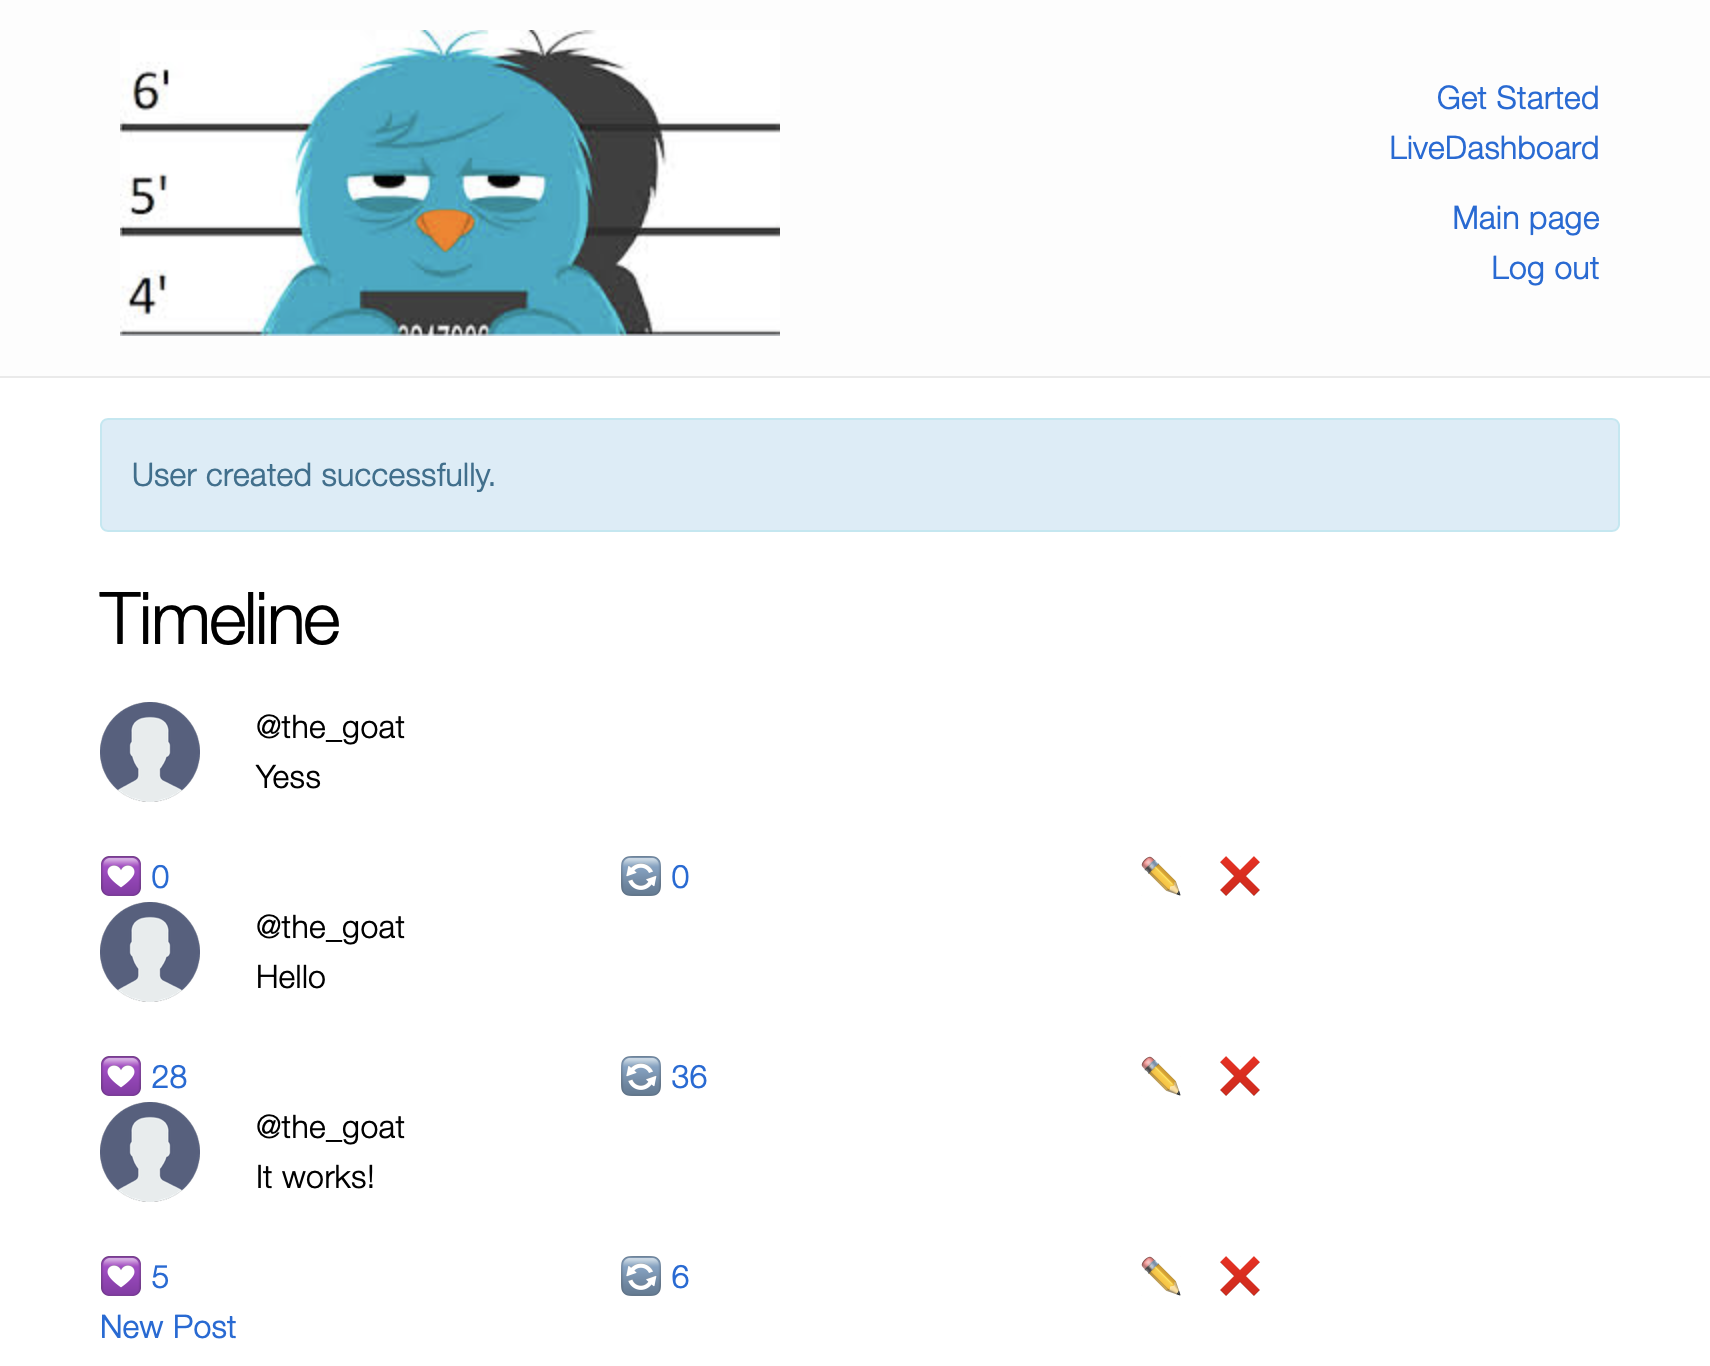
\includegraphics[width=\linewidth]{figures/created_user.png}
		\caption{New user created}
		\label{fig:user}
	\end{minipage}
	\hfill
	\begin{minipage}[b]{0.45\textwidth}
		\centering
		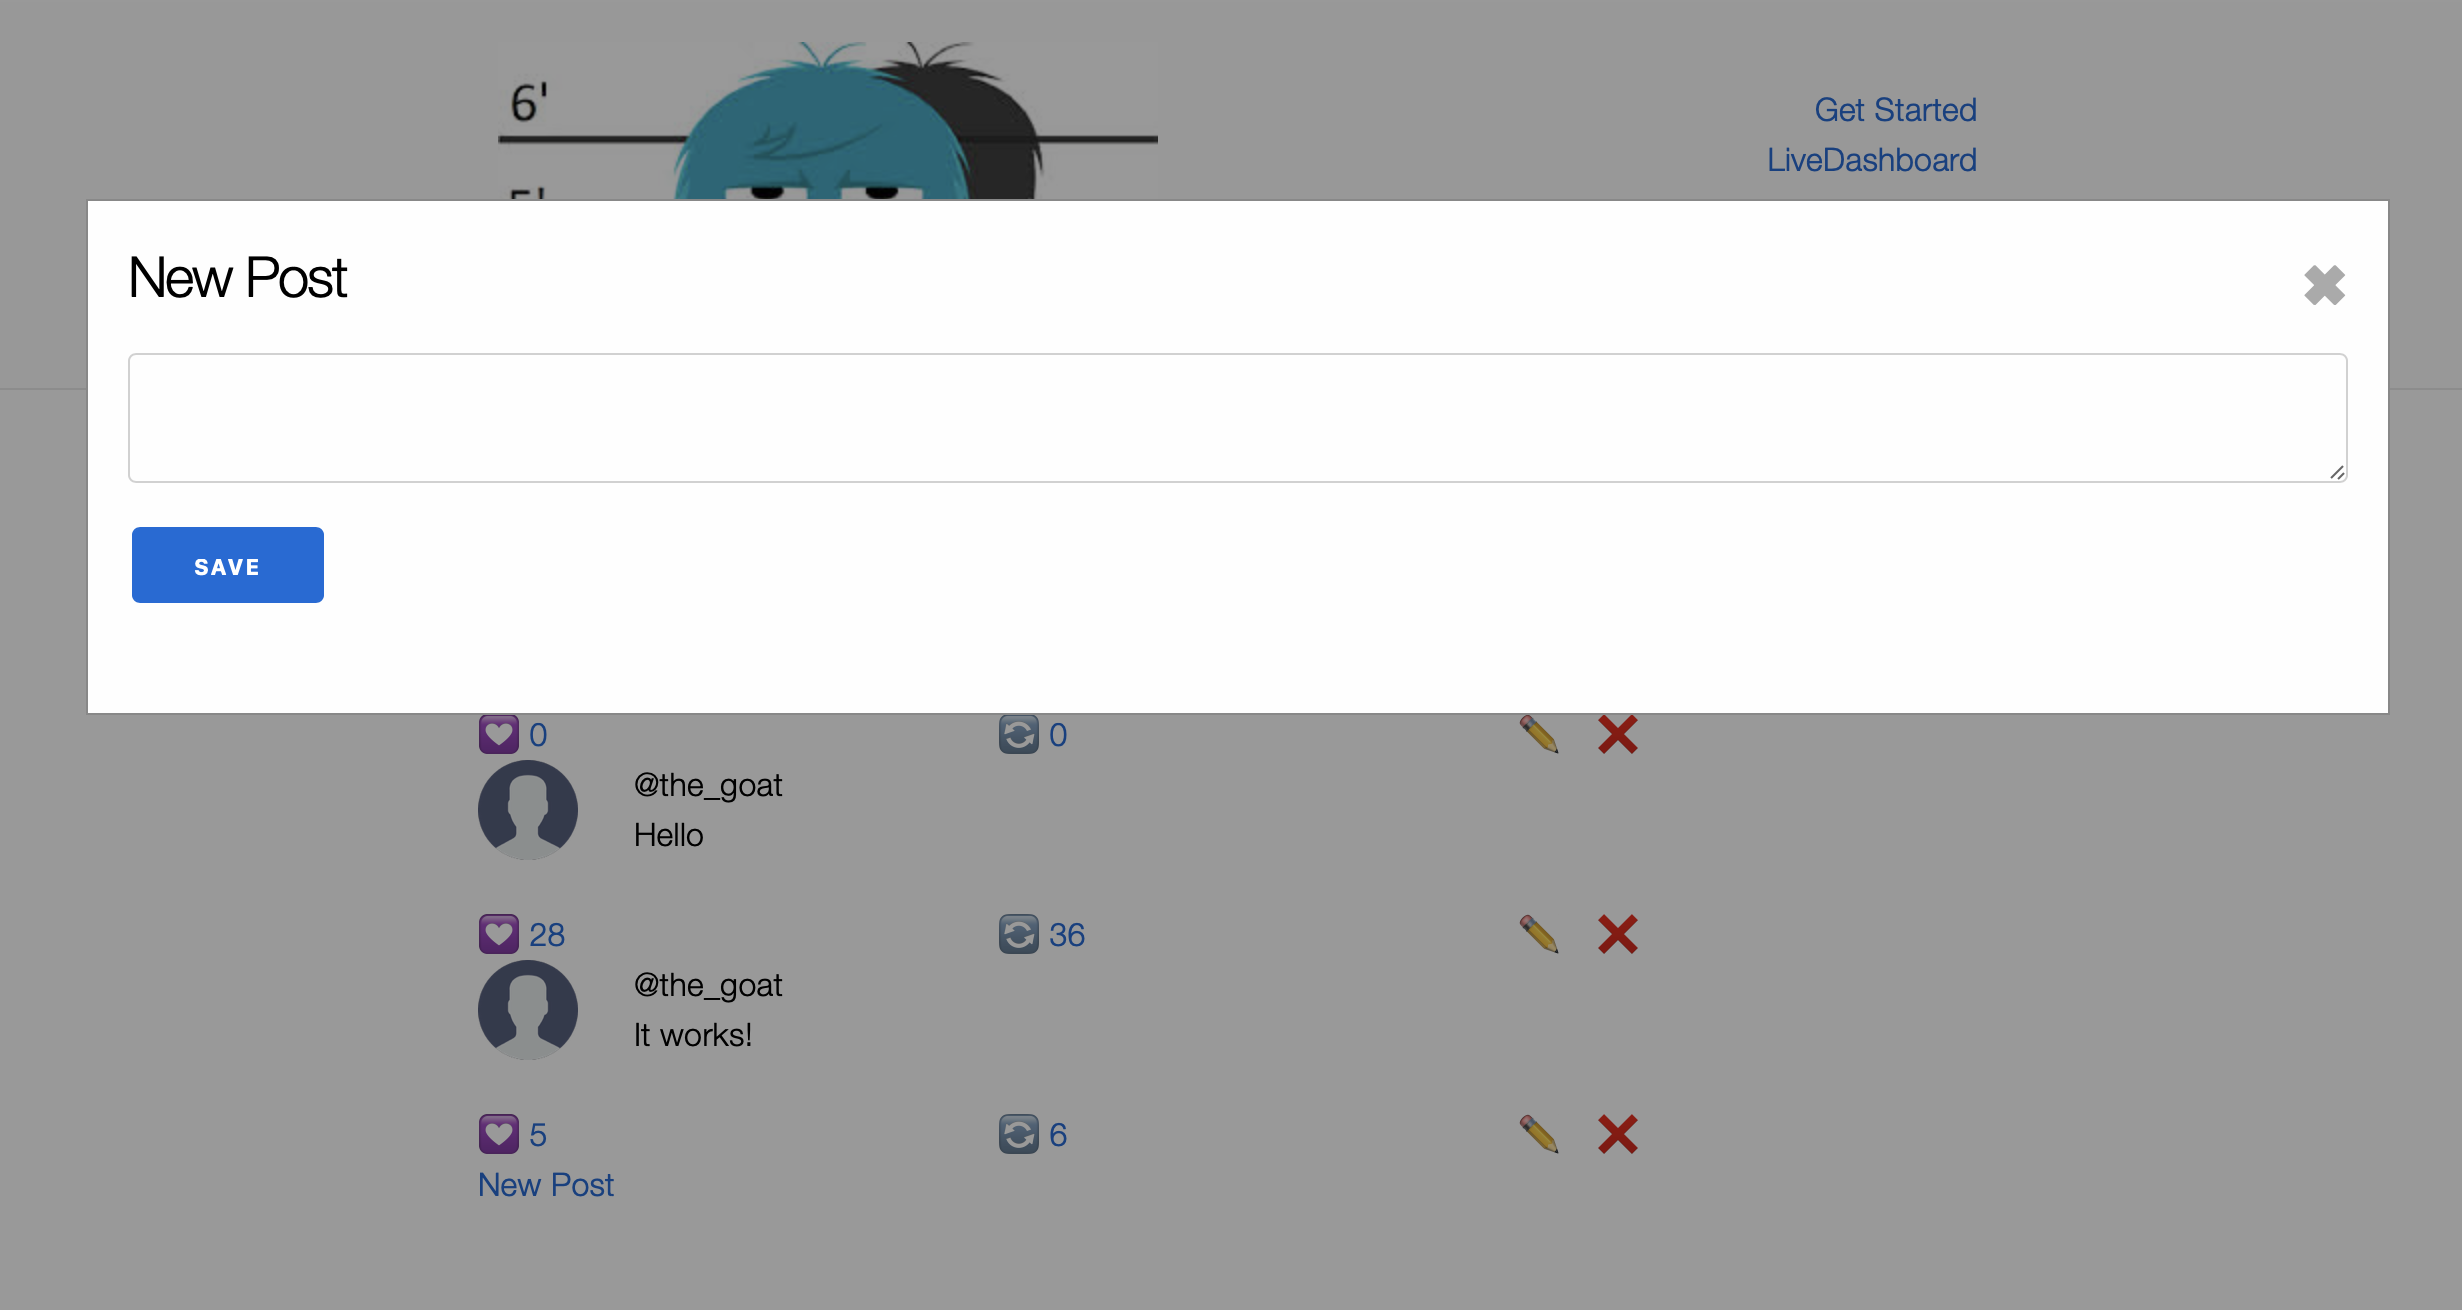
\includegraphics[width=\linewidth]{figures/new_post.png}
		\caption{Create new post}
		\label{fig:np}
	\end{minipage}

\end{figure}


\begin{figure}[htbp]
	\centering
	
	\begin{minipage}[b]{0.45\textwidth}
		\centering
		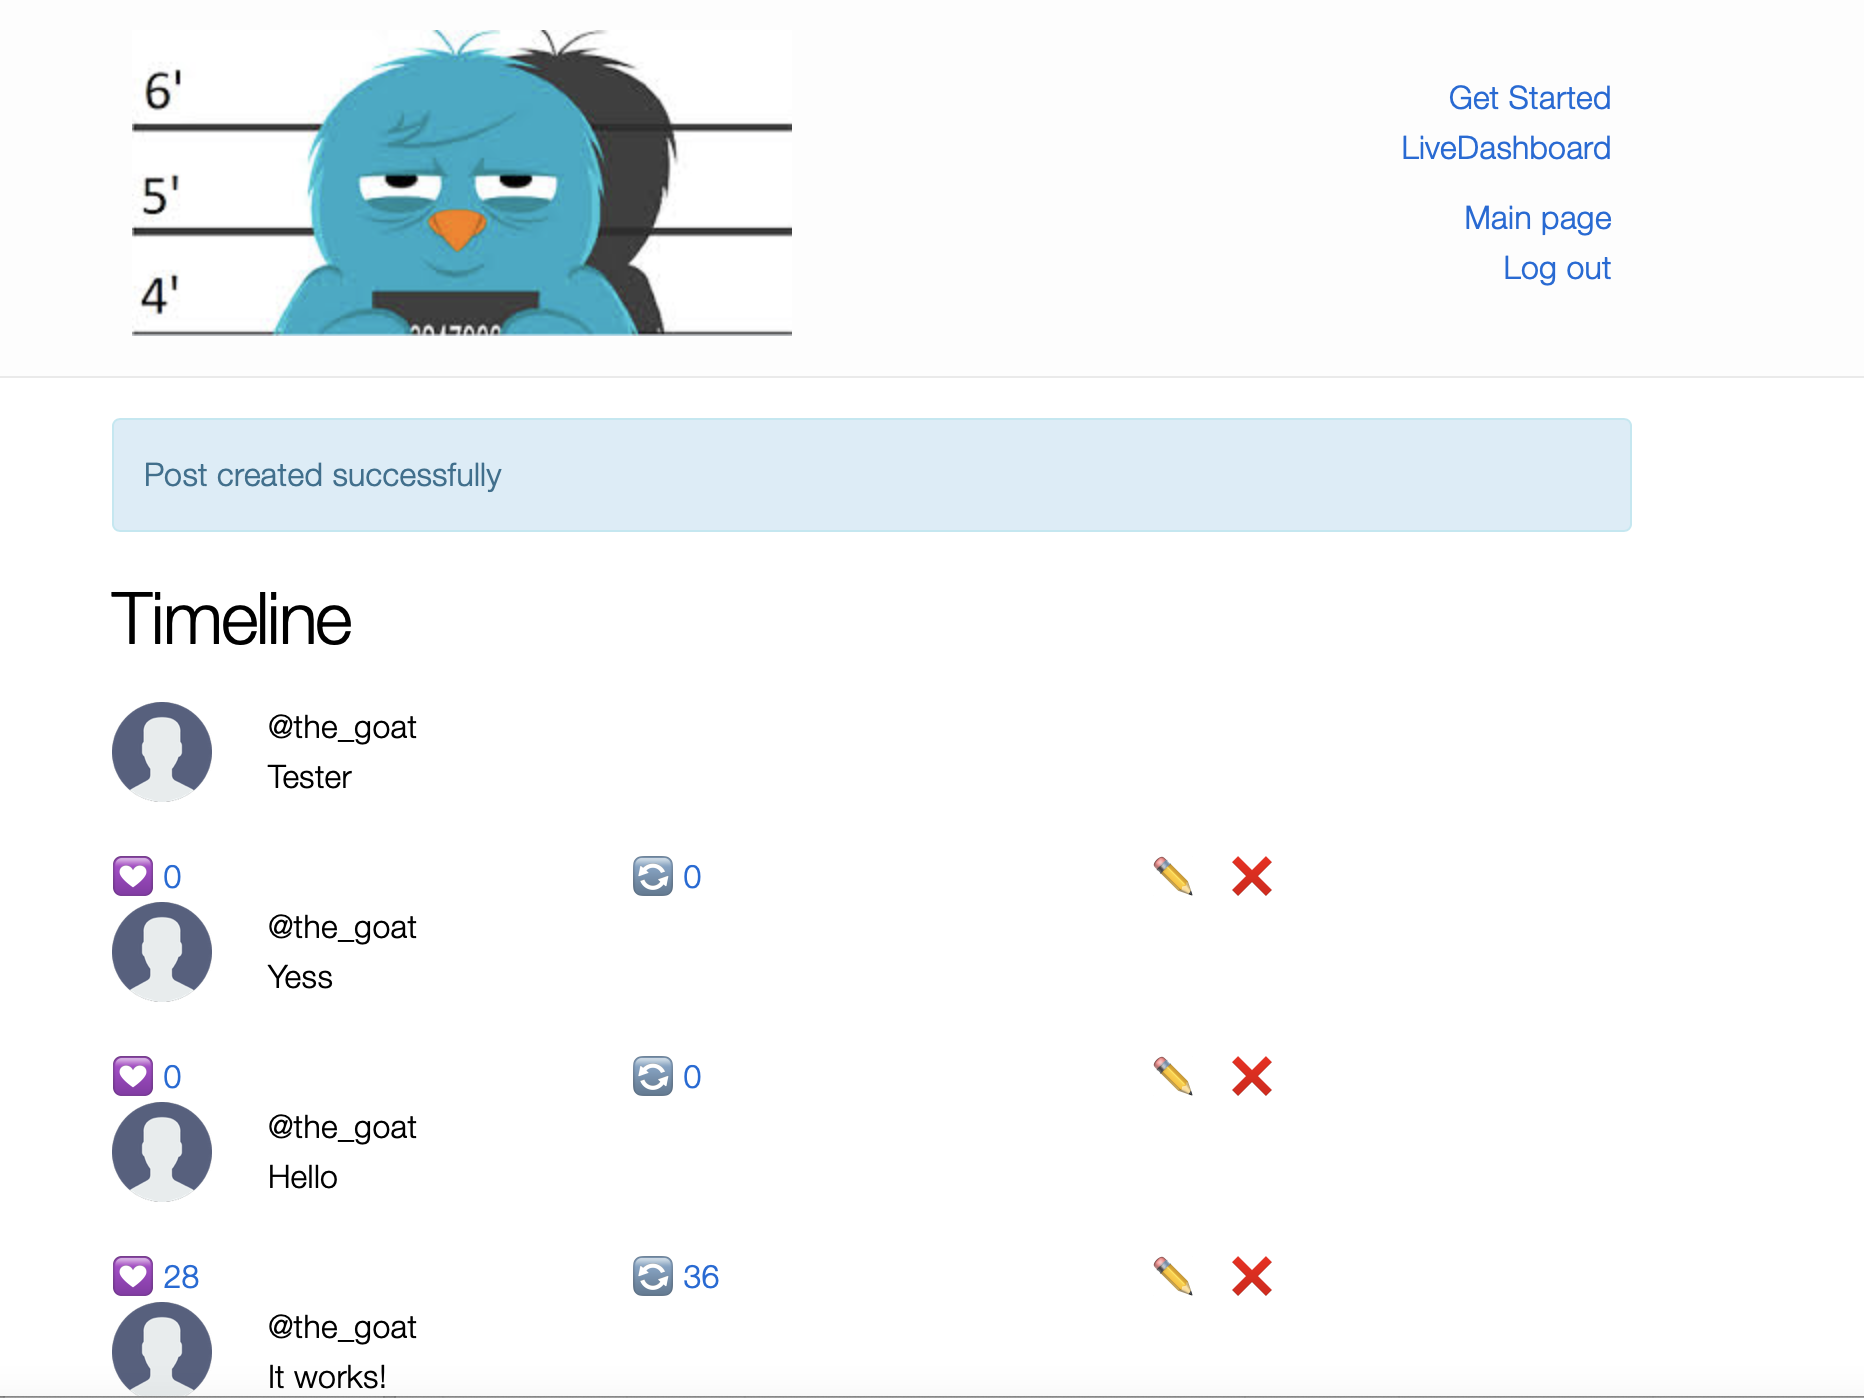
\includegraphics[width=\linewidth]{figures/post.png}
		\caption{Post}
		\label{fig:post}
	\end{minipage}
	\hfill
	\begin{minipage}[b]{0.45\textwidth}
		\centering
		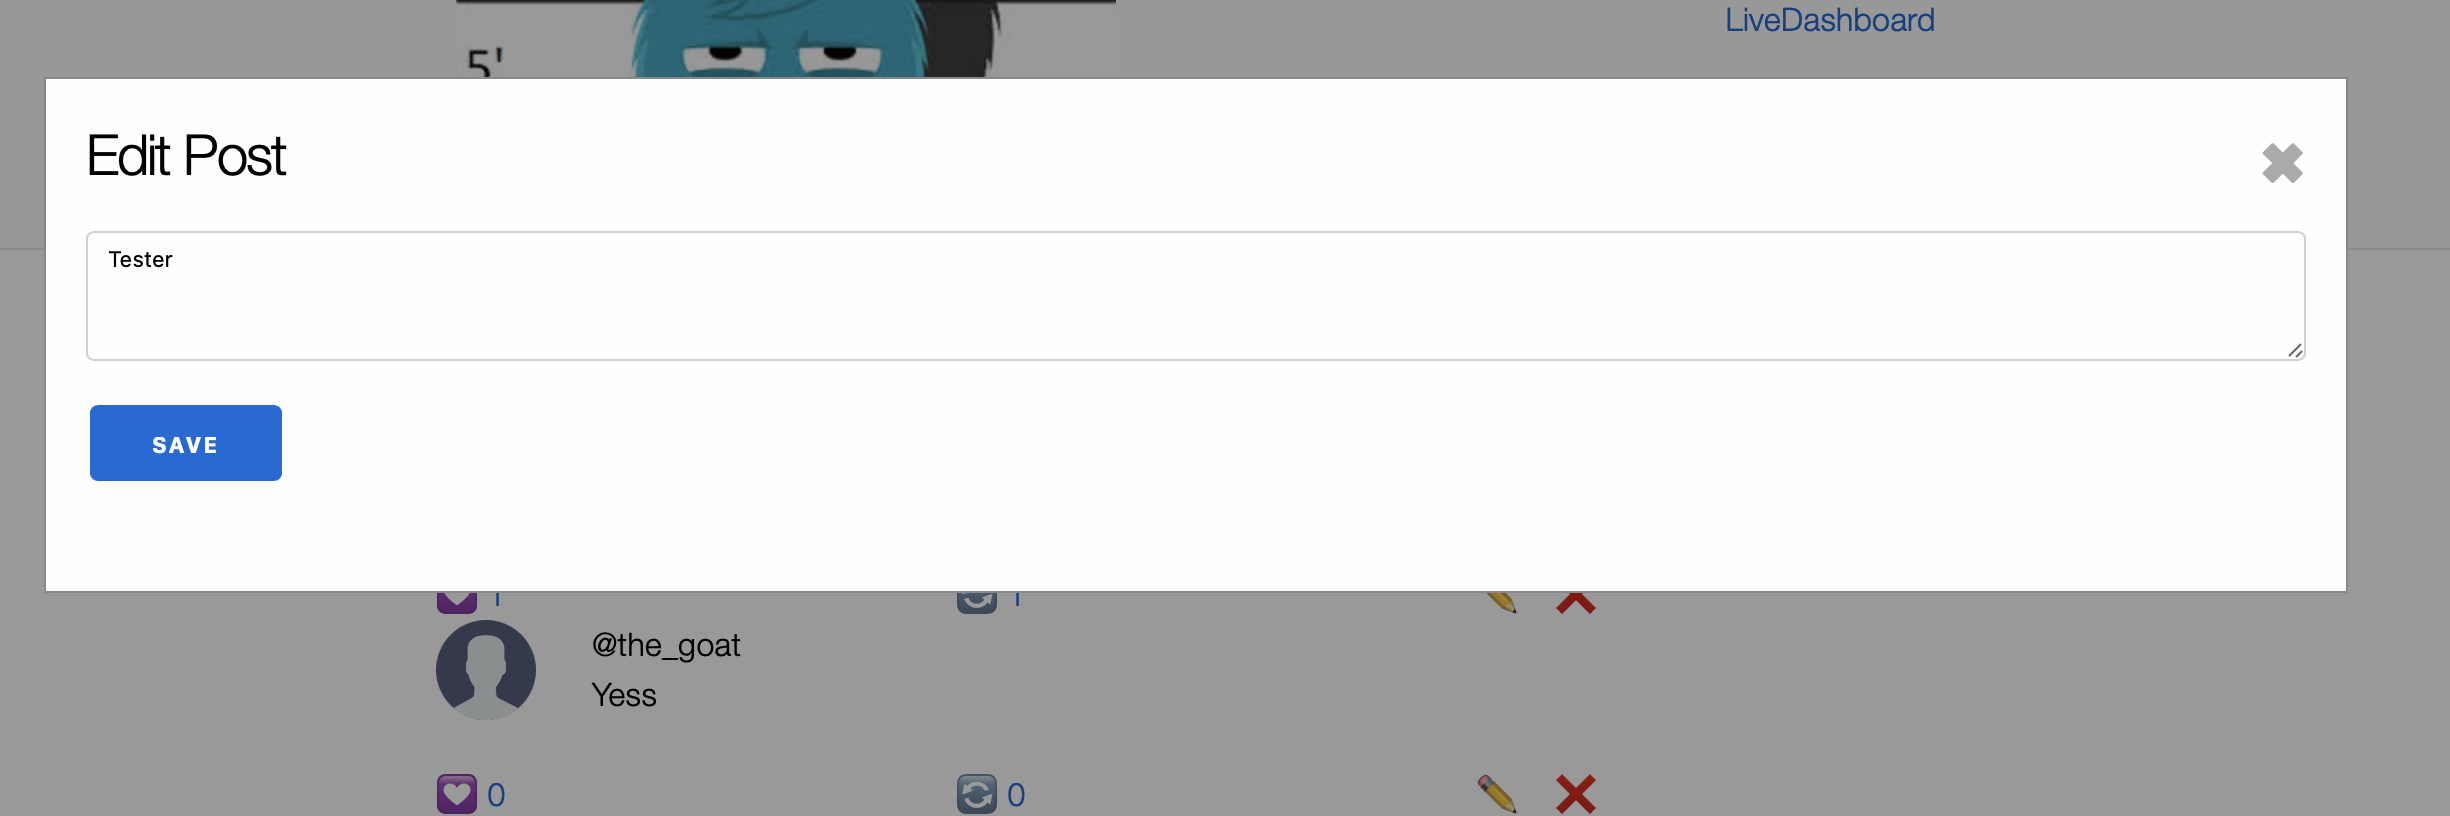
\includegraphics[width=\linewidth]{figures/edit.png}
		\caption{Edit post}
		\label{fig:edit}
	\end{minipage}

\end{figure}

\begin{figure}[htbp]
	\centering
	
	\begin{minipage}[b]{0.45\textwidth}
		\centering
		
\includegraphics[width=\linewidth]{figures/delete.png}
		\caption{Delete post notification}
		\label{fig:delete}
	\end{minipage}
	\hfill
	\begin{minipage}[b]{0.45\textwidth}
		\centering
		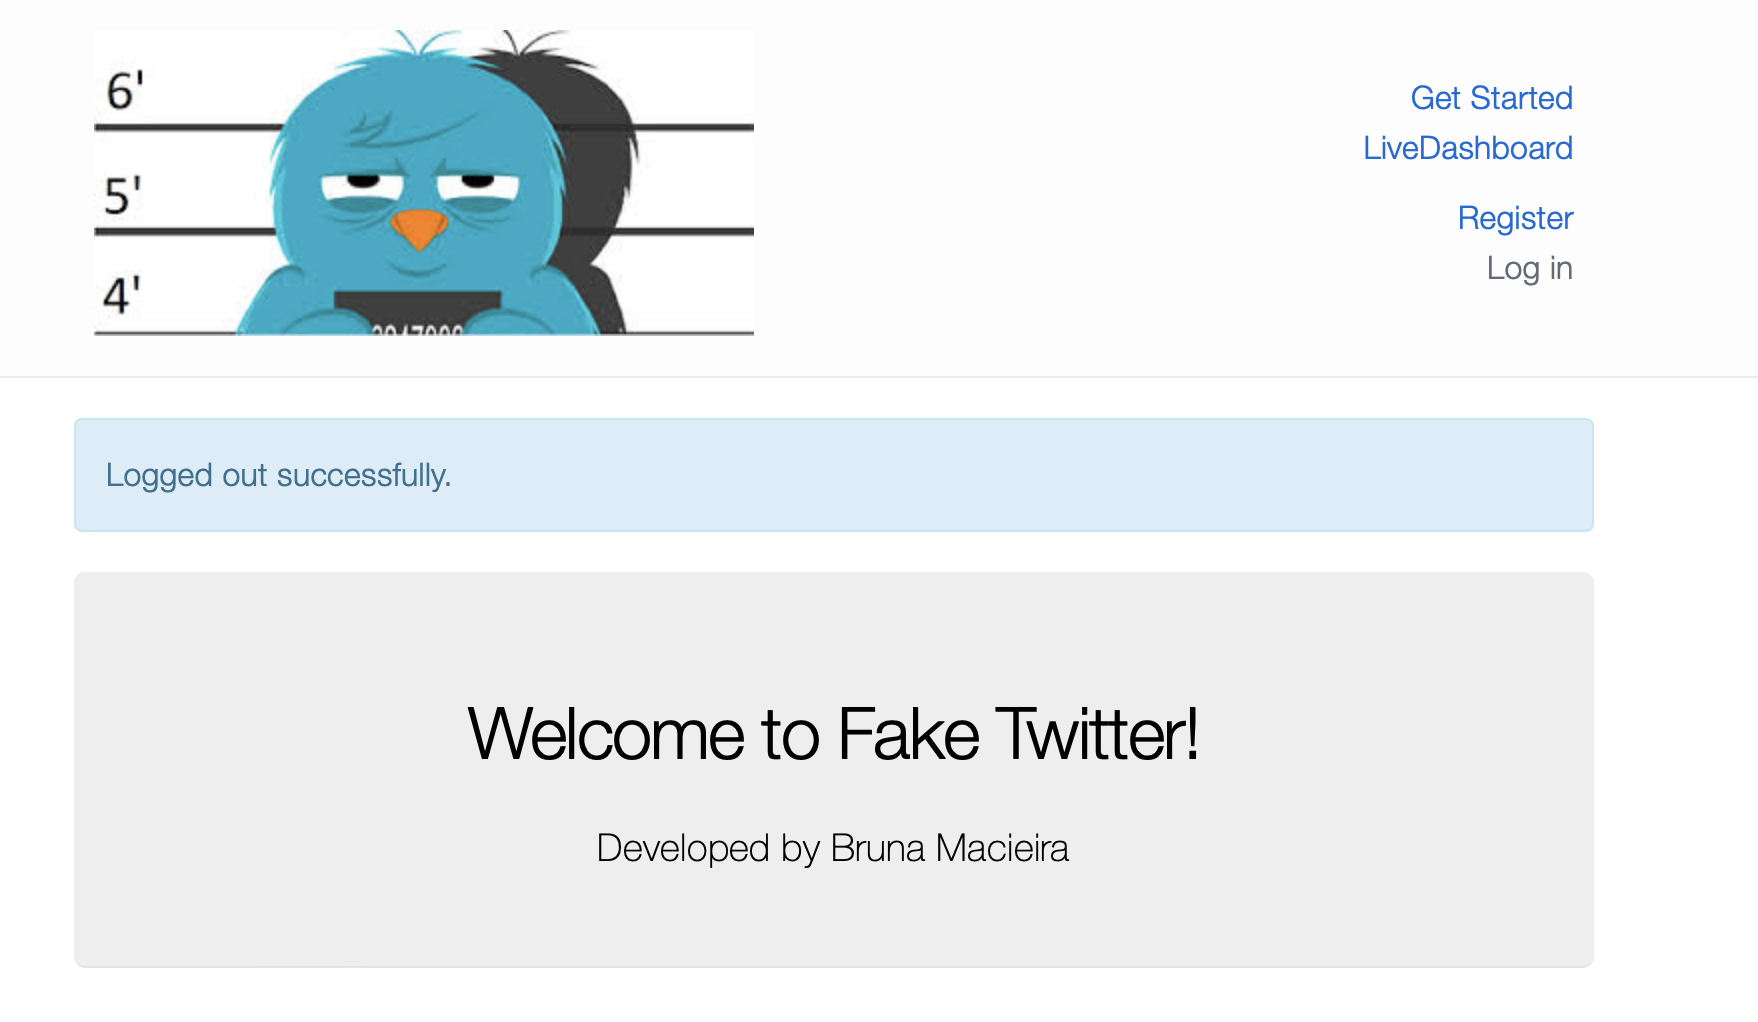
\includegraphics[width=\linewidth]{figures/logout.png}
		\caption{Logout}
		\label{fig:logout}
	\end{minipage}

\end{figure}



Users' information, like posts, email and so on, can be checked on tools like PG-Admin (see section \ref{post}). Regarding a tip given by a Yarilabs employee, \href{https://eggerapps.at/postico2/}{\textit{Postico}}\footnote{For a further understanding of Postico, please check: https://eggerapps.at/postico2/} was used.

\begin{figure}[htbp]
	\centering
	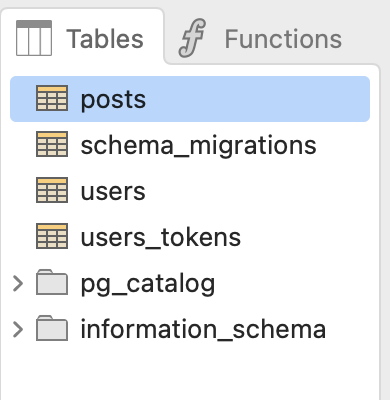
\includegraphics[scale=0.5]{figures/postico.png}  % largura percentual
	\caption{Postico's data}
	\label{fig:postico}
\end{figure}


\section{Tentacat} \label{tentacat}

\textit{Tentacat} is a \textit{GitHub wrapper} for Elixir. It allows Elixir developers to seamlessly integrate their applications with GitHub's extensive functionality and data.

With Tentacat, various operations can be performed on GitHub repositories, issues, pull requests, organizations, users, and more. It simplifies the process of authenticating with the GitHub API, making requests, and handling responses, providing a convenient interface for building GitHub-related functionality into Elixir applications.

Tentacat leverages the power of Elixir's concurrency model and functional programming paradigm to offer efficient and reliable interactions with the GitHub API. It provides a set of expressive and intuitive functions to query and manipulate GitHub resources, making it easier to retrieve information, create or update repositories, manage issues, and perform other GitHub-related tasks programmatically.

Some key features and benefits of Tentacat include:

\begin{itemize}
    \item \textit{GitHub API Integration}: Tentacat seamlessly integrates with the GitHub API, allowing developers to interact with GitHub's vast ecosystem of features and data.
    \item \textit{Authentication}: Tentacat provides authentication mechanisms, including personal access tokens and OAuth, to securely access the GitHub API on behalf of users or applications.
    \item \textit{Resource Operations}: Tentacat offers a rich set of functions to perform operations on GitHub resources. Developers can create, read, update, and delete repositories, manage issues and pull requests, work with organizations and users, and more.
    \item \textit{Error Handling}: Tentacat handles API errors and provides meaningful error messages and exceptions, making it easier to handle and recover from potential issues.
    \item \textit{Concurrent Requests}: Built on top of Elixir's concurrency model, Tentacat allows developers to make concurrent requests to the GitHub API, improving performance and responsiveness of applications.
    \item \textit{Extensibility}: Tentacat is designed to be extensible, allowing customization and extend its functionality as per the application's requirements.
    \cite{tentacat}
\end{itemize}

Tentacat can be a valuable asset in Elixir development toolkit and it sure was when it came to Dharma Network.

\begin{figure}[htbp]
	\centering
	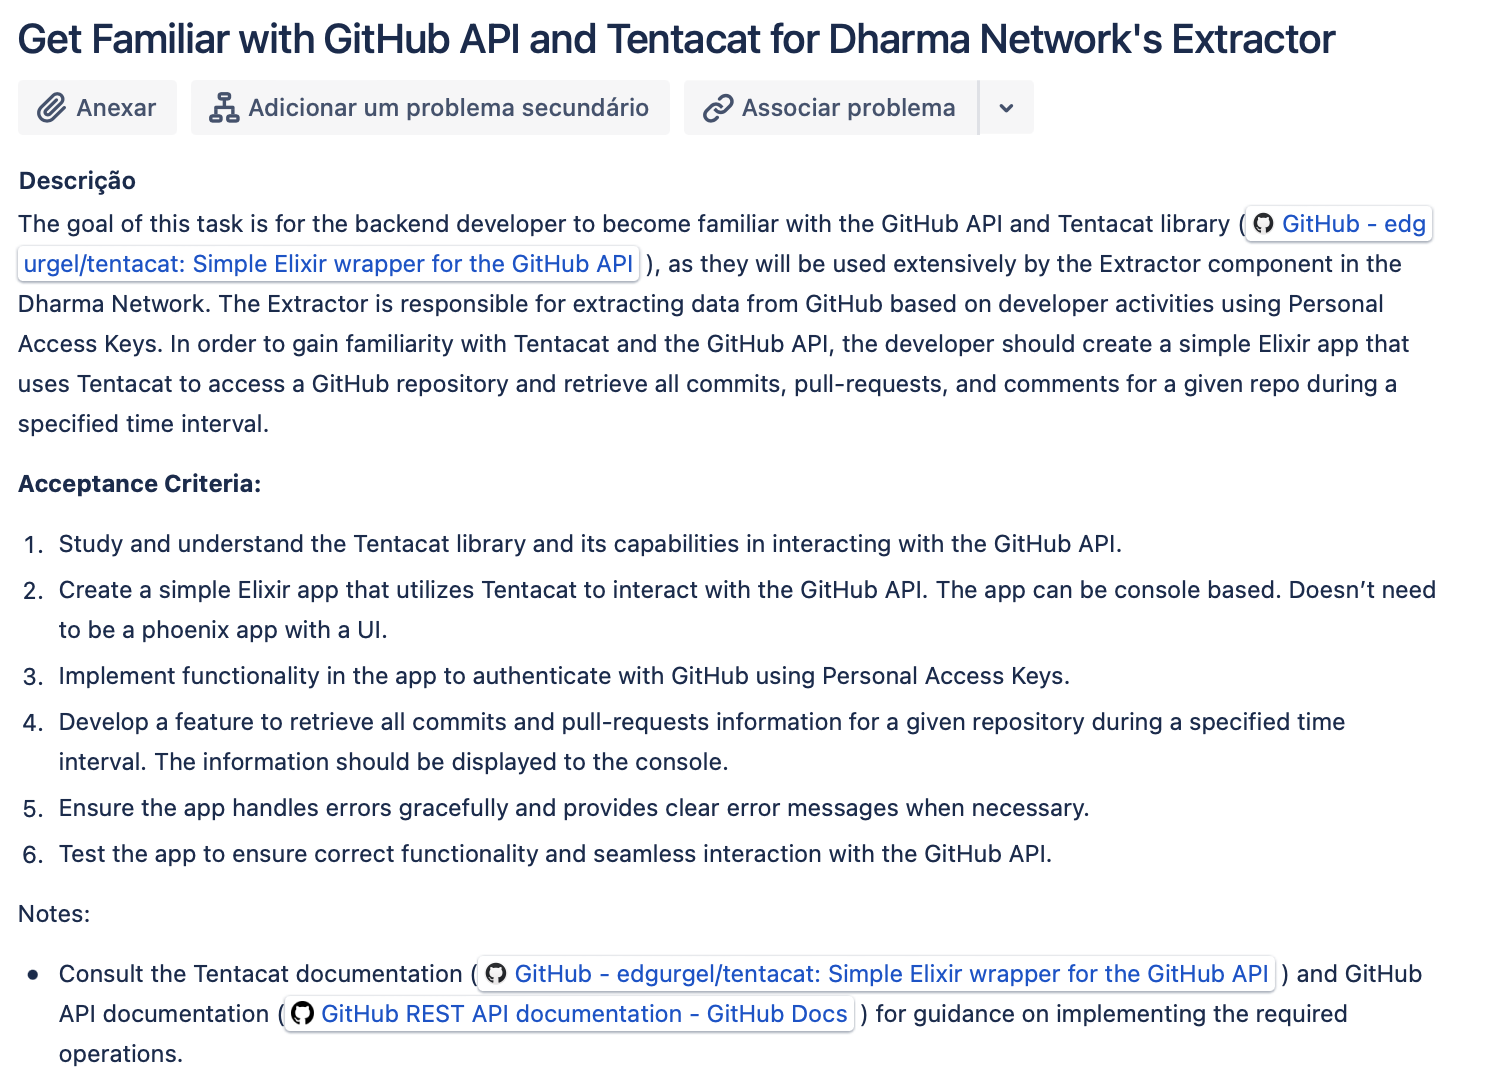
\includegraphics[scale=0.5]{figures/ticket.png}  % largura percentual
	\caption{Tentacat's ticket}
	\label{fig:ticket}
\end{figure}

As seen on the figure \ref{fig:ticket}, it was up for the developer to become familiar with GitHub API (see \ref{github}), since it's a key resource to be consumed by Dharma Network.

This component, in similarity to the previous study objects, took a vast learning period, as it was of extreme importance.\newline

Since there's not a lot of resources online about this tool, the available ones were scrupulously analyzed. The main resources were the \href{https://github.com/edgurgel/tentacat}{\textit{Tentacat source code}}\footnote{To check Tentacat's source code, please check: https://github.com/edgurgel/tentacat} and \href{https://hexdocs.pm/tentacat/readme.html}{\textit{Tentacat Hex files}}\footnote{To check Tentacat's Hex files, please check: https://hexdocs.pm/tentacat/readme.html}. \newline

Once the basics of Tentacat and GitHub API were understood, a project named \texttt{tentahub} (Tentacat + GitHub) was created.

\begin{figure}[htbp]
	\centering
	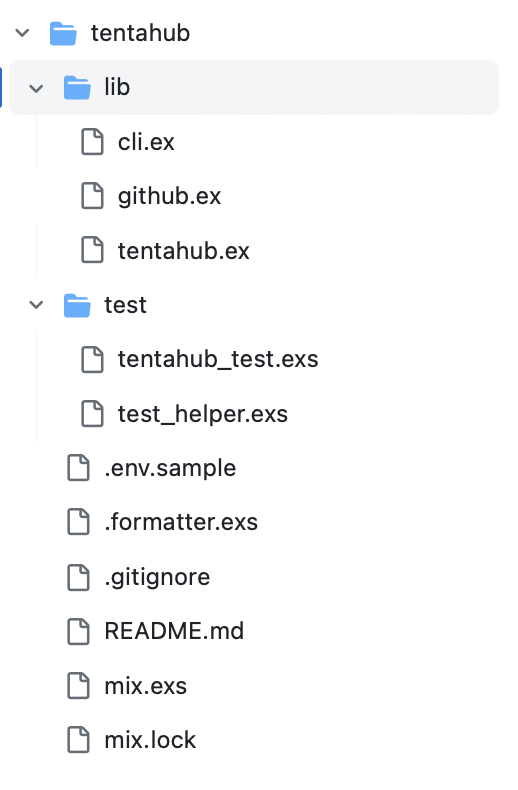
\includegraphics[scale=0.5]{figures/tentahub.png}  % largura percentual
	\caption{Tentacat's files}
	\label{fig:tent}
\end{figure}

As seen on image \ref{fig:tent}, the project's main folder is called \texttt{lib}. This folder contains 3 files, responsible for: connecting to the GitHub API, extracting the data and running the application. Also, the file \texttt{env.sample} contains then necessary user information to fetch the GitHub data, which is confidential, and is why, before running the program, the command {
\newcommand{\shellcmd}[1]{\\\indent\indent\texttt{\footnotesize\# #1}\\}
  \shellcmd{cp .env.sample .env}
}should be ran, in order to create an editable file where confidential information can be stored.\newline

Then, the command {
\newcommand{\shellcmd}[1]{\\\indent\indent\texttt{\footnotesize\# #1}\\}
  \shellcmd{mix guardian.gen.secret}
} should be compiled in order to generate a JWT secret, necessary for the execution of the application.\newline

That information should be stored here, substituting the information between brackets:

\begin{lstlisting}[language=Erlang, caption={Setup of.env.sample}]
export GITHUB_TOKEN=<your-token>
export GITHUB_OWNER=<repository-owner>
export GITHUB_REPO=<repository-name>
export SINCE_DATE=<start-date>
export UNTIL_DATE=<end-date>
\end{lstlisting}

Analyzing the \texttt{tentahub} project, it's shown:

\begin{lstlisting}[language=Erlang, caption={Configuration of github.ex}]
    defmodule GitHub do
  def get_commits(client, owner, repo, since, until) do
    filters = [since: since, until: until, per_page: 100]
    Tentacat.Commits.filter(client, owner, repo, filters)
  end

  def get_pull_requests(client, owner, repo, since, until) do
    filters = [state: "all", sort: "created", direction: "asc", since: since, until: until, per_page: 100]
    Tentacat.Pulls.filter(client, owner, repo, filters)
  end

  def get_comments(client, owner, repo, since, until) do
    Tentacat.Issues.Comments.list_all(client, owner, repo)
  end
end
\end{lstlisting} 

\begin{lstlisting}[language=Erlang, caption={Setup of tentahub.ex}]
    defmodule Tentahub do
  def run do
    Cli.run()
  end
end
\end{lstlisting}


\begin{lstlisting}[language=Erlang, caption={Configuration of cli.ex}]
    defmodule Cli do
  def run do
    token = System.get_env("GITHUB_TOKEN")
    owner = System.get_env("GITHUB_OWNER")
    repo = System.get_env("GITHUB_REPO")
    since = System.get_env("SINCE_DATE")
    until = System.get_env("UNTIL_DATE")

    client = Tentacat.Client.new(%{access_token: token})

    commits = GitHub.get_commits(client, owner, repo, since, until)
    pull_requests = GitHub.get_pull_requests(client, owner, repo, since, until)
    comments = GitHub.get_comments(client, owner, repo, since, until)

    IO.puts "-----------------------Commits:------------------------------"
    IO.inspect commits

    IO.puts "-----------------------Pull requests:------------------------"
    IO.inspect pull_requests

    IO.puts "-----------------------Comments:-----------------------------"
    IO.inspect comments
  end
end
\end{lstlisting}

Although it might seem a simple application, the testing took awhile, since the correct information wasn't being retrieved.\newline

While doing this project, a better insight was uncovered regarding the structure of Github API. For instance, to retrieve specific information from pull requests \label{issue}, like to filter them by \texttt{since} date, the module \texttt{Pulls} is not enough; after some research, it was found that the module \texttt{Issues} was just right, since a pull request is always an issue, but an issue might not always be a pull request. Plus, it allows the filtering by \texttt{since} date.\newline

With the cessation of this project, we took a step closer to the main project.


\section{GitHub API} \label{github}

The GitHub API is a powerful application programming interface that allows developers to interact with the resources and data of the GitHub platform. As a leading platform for source code hosting and development collaboration, GitHub provides a rich set of APIs that enable developers to automate workflows, integrate with other tools, and build applications that leverage GitHub's functionality.\newline

With the GitHub API, developers can perform a wide range of operations, such as creating and managing repositories, accessing and manipulating issues and pull requests, retrieving user information, and much more. The API can programmatically interact with GitHub's features and integrate them into applications, tools, or scripts.\newline

The GitHub API follows the principles of REST (Representational State Transfer) and provides endpoints that return data in JSON format. It supports various authentication methods, including personal access tokens and OAuth, ensuring secure access to the API's capabilities.\newline

By leveraging the GitHub API, developers gain enhanced control and flexibility in managing their repositories, automating repetitive tasks, integrating with external services, and gaining insights into their development processes.\newline

When it comes to its usage in Dharma Network, it's a key resource, since the entire algorithm of the platform depends on it (as for the first release).\newline

As seen above (see section \ref{tentacat}), it was inserted onto the \texttt{tentahub} application, in order to collect data from a GitHub repository. 

The connection and filtering was accomplished by following the \href{https://docs.github.com/pt/rest/quickstart?apiVersion=2022-11-28}{\textbf{GitHub documentation}}\footnote{To check GitHub API's documentation, please check: https://docs.github.com/pt/rest/quickstart?apiVersion=2022-11-28}.

\section{Bug Hunting on Durga}\label{bug}

Following the training of such concepts, it was time to follow for the main project: Dharma Network. \newline
Dharma Network is divided into 3 categories: \textit{Rudra}, the web application frontend; \textit{Durga}, the backend services; and \textit{Algodex}, the Algorand SDK developed by Dharma Network. The exploited one in this section will be \textit{Durga}, the backend project.\newline

The first interaction with Durga was meant to understand its structure and components, which will be presented next chapter (see chapter \ref{chap:chap4}). \newline
One easy way to better understand the program and what it retrieves is by running the code. However, that was not possible.\newline

Dharma Network's project had been untouched for a year, which, with all the upgrades on the dependencies and languages, led to its break.\newline

Upon encountering this issue, the team invested time to uncover its cause. The answer was found in the ErlPort dependency.\newline

\href{https://github.com/erlport/erlport}{\textit{ErlPort}}\footnote{For a further understanding of ErlPort, please check: https://github.com/erlport/erlport} serves as a crucial interface between the Elixir components and the Python workers executing the Algorand Python SDK, which performs cryptographic functions not yet implemented in Algodex.

Updating ErlPort was necessary to prevent project compromise, but the process posed a risk to other dependencies. The team proceeded cautiously, opting for a manual code update to mitigate this risk.\newline

Another important consideration was the version of Python in use. If the version was more recent than what the existing code was built upon, adjustments were required to ensure compatibility and prevent further issues.\newline

After identifying the problematic code snippets and performing the necessary updates, the code was ready for execution, clearing the path for further project development.